% Created by tikzDevice version 0.12.6 on 2026-07-16 13:12:42
% !TEX encoding = UTF-8 Unicode
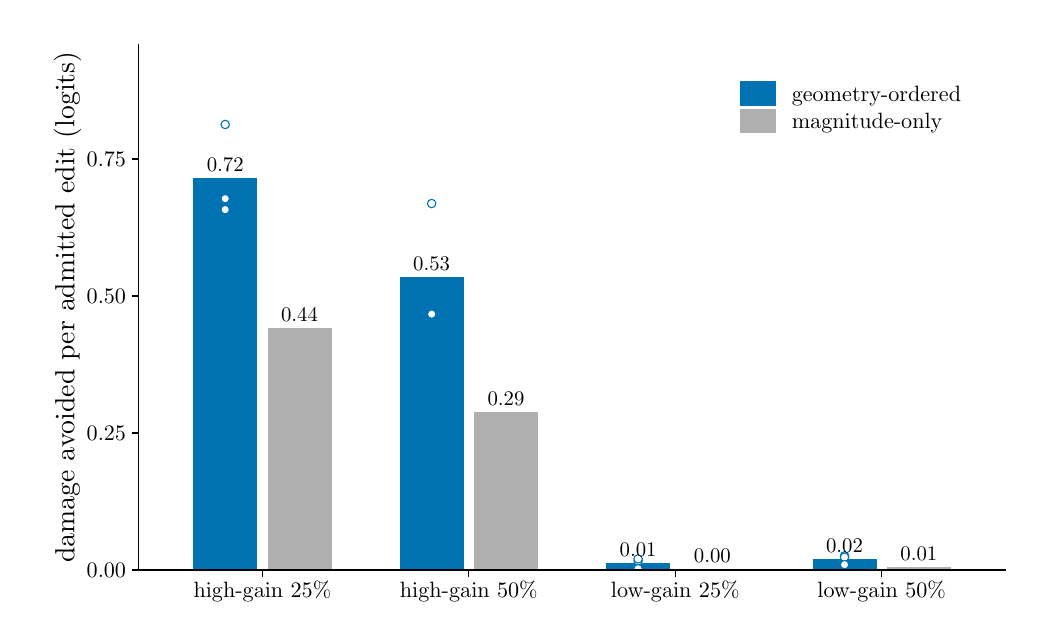
\begin{tikzpicture}[x=1pt,y=1pt]
\definecolor{fillColor}{RGB}{255,255,255}
\path[use as bounding box,fill=fillColor,fill opacity=0.00] (0,0) rectangle (361.35,209.58);
\begin{scope}
\path[clip] (  0.00,  0.00) rectangle (361.35,209.58);
\definecolor{drawColor}{RGB}{255,255,255}
\definecolor{fillColor}{RGB}{255,255,255}

\path[draw=drawColor,line width= 0.5pt,line join=round,line cap=round,fill=fillColor] (  0.00,  0.00) rectangle (361.35,209.58);
\end{scope}
\begin{scope}
\path[clip] ( 40.05, 13.56) rectangle (353.35,203.58);
\definecolor{fillColor}{RGB}{255,255,255}

\path[fill=fillColor] ( 40.05, 13.56) rectangle (353.35,203.58);
\definecolor{fillColor}{RGB}{0,114,178}

\path[fill=fillColor] ( 59.82, 13.56) rectangle ( 82.94,155.41);
\definecolor{fillColor}{gray}{0.69}

\path[fill=fillColor] ( 86.67, 13.56) rectangle (109.80,101.18);
\definecolor{fillColor}{RGB}{0,114,178}

\path[fill=fillColor] (134.41, 13.56) rectangle (157.54,119.34);
\definecolor{fillColor}{gray}{0.69}

\path[fill=fillColor] (161.27, 13.56) rectangle (184.39, 70.81);
\definecolor{fillColor}{RGB}{0,114,178}

\path[fill=fillColor] (209.01, 13.56) rectangle (232.13, 16.20);
\definecolor{fillColor}{gray}{0.69}

\path[fill=fillColor] (235.86, 13.56) rectangle (258.99, 13.82);
\definecolor{fillColor}{RGB}{0,114,178}

\path[fill=fillColor] (283.60, 13.56) rectangle (306.73, 17.51);
\definecolor{fillColor}{gray}{0.69}

\path[fill=fillColor] (310.46, 13.56) rectangle (333.58, 14.65);
\definecolor{drawColor}{RGB}{0,114,178}
\definecolor{fillColor}{RGB}{255,255,255}

\path[draw=drawColor,line width= 0.4pt,line join=round,line cap=round,fill=fillColor] ( 71.38,174.60) circle (  1.53);

\path[draw=drawColor,line width= 0.4pt,line join=round,line cap=round,fill=fillColor] ( 71.38,147.79) circle (  1.53);

\path[draw=drawColor,line width= 0.4pt,line join=round,line cap=round,fill=fillColor] ( 71.38,143.83) circle (  1.53);

\path[draw=drawColor,line width= 0.4pt,line join=round,line cap=round,fill=fillColor] (145.98,146.03) circle (  1.53);

\path[draw=drawColor,line width= 0.4pt,line join=round,line cap=round,fill=fillColor] (145.98,105.93) circle (  1.53);

\path[draw=drawColor,line width= 0.4pt,line join=round,line cap=round,fill=fillColor] (145.98,106.07) circle (  1.53);

\path[draw=drawColor,line width= 0.4pt,line join=round,line cap=round,fill=fillColor] (220.57, 16.91) circle (  1.53);

\path[draw=drawColor,line width= 0.4pt,line join=round,line cap=round,fill=fillColor] (220.57, 17.62) circle (  1.53);

\path[draw=drawColor,line width= 0.4pt,line join=round,line cap=round,fill=fillColor] (220.57, 14.08) circle (  1.53);

\path[draw=drawColor,line width= 0.4pt,line join=round,line cap=round,fill=fillColor] (295.17, 18.73) circle (  1.53);

\path[draw=drawColor,line width= 0.4pt,line join=round,line cap=round,fill=fillColor] (295.17, 18.24) circle (  1.53);

\path[draw=drawColor,line width= 0.4pt,line join=round,line cap=round,fill=fillColor] (295.17, 15.54) circle (  1.53);
\definecolor{drawColor}{RGB}{0,0,0}

\node[text=drawColor,anchor=base,inner sep=0pt, outer sep=0pt, scale=  0.75] at ( 71.38,157.75) {0.72};

\node[text=drawColor,anchor=base,inner sep=0pt, outer sep=0pt, scale=  0.75] at ( 98.23,103.52) {0.44};

\node[text=drawColor,anchor=base,inner sep=0pt, outer sep=0pt, scale=  0.75] at (145.98,121.67) {0.53};

\node[text=drawColor,anchor=base,inner sep=0pt, outer sep=0pt, scale=  0.75] at (172.83, 73.14) {0.29};

\node[text=drawColor,anchor=base,inner sep=0pt, outer sep=0pt, scale=  0.75] at (220.57, 18.54) {0.01};

\node[text=drawColor,anchor=base,inner sep=0pt, outer sep=0pt, scale=  0.75] at (247.42, 16.16) {0.00};

\node[text=drawColor,anchor=base,inner sep=0pt, outer sep=0pt, scale=  0.75] at (295.17, 19.84) {0.02};

\node[text=drawColor,anchor=base,inner sep=0pt, outer sep=0pt, scale=  0.75] at (322.02, 16.99) {0.01};
\end{scope}
\begin{scope}
\path[clip] (  0.00,  0.00) rectangle (361.35,209.58);
\definecolor{drawColor}{RGB}{0,0,0}

\path[draw=drawColor,line width= 0.5pt,line join=round,line cap=rect] ( 40.05, 13.56) --
	( 40.05,203.58);
\end{scope}
\begin{scope}
\path[clip] (  0.00,  0.00) rectangle (361.35,209.58);
\definecolor{drawColor}{RGB}{0,0,0}

\node[text=drawColor,anchor=base east,inner sep=0pt, outer sep=0pt, scale=  0.80] at ( 35.55, 10.81) {0.00};

\node[text=drawColor,anchor=base east,inner sep=0pt, outer sep=0pt, scale=  0.80] at ( 35.55, 60.31) {0.25};

\node[text=drawColor,anchor=base east,inner sep=0pt, outer sep=0pt, scale=  0.80] at ( 35.55,109.81) {0.50};

\node[text=drawColor,anchor=base east,inner sep=0pt, outer sep=0pt, scale=  0.80] at ( 35.55,159.31) {0.75};
\end{scope}
\begin{scope}
\path[clip] (  0.00,  0.00) rectangle (361.35,209.58);
\definecolor{drawColor}{RGB}{0,0,0}

\path[draw=drawColor,line width= 0.5pt,line join=round] ( 37.55, 13.56) --
	( 40.05, 13.56);

\path[draw=drawColor,line width= 0.5pt,line join=round] ( 37.55, 63.06) --
	( 40.05, 63.06);

\path[draw=drawColor,line width= 0.5pt,line join=round] ( 37.55,112.56) --
	( 40.05,112.56);

\path[draw=drawColor,line width= 0.5pt,line join=round] ( 37.55,162.06) --
	( 40.05,162.06);
\end{scope}
\begin{scope}
\path[clip] (  0.00,  0.00) rectangle (361.35,209.58);
\definecolor{drawColor}{RGB}{0,0,0}

\path[draw=drawColor,line width= 0.5pt,line join=round,line cap=rect] ( 40.05, 13.56) --
	(353.35, 13.56);
\end{scope}
\begin{scope}
\path[clip] (  0.00,  0.00) rectangle (361.35,209.58);
\definecolor{drawColor}{RGB}{0,0,0}

\path[draw=drawColor,line width= 0.5pt,line join=round] ( 84.81, 11.06) --
	( 84.81, 13.56);

\path[draw=drawColor,line width= 0.5pt,line join=round] (159.40, 11.06) --
	(159.40, 13.56);

\path[draw=drawColor,line width= 0.5pt,line join=round] (234.00, 11.06) --
	(234.00, 13.56);

\path[draw=drawColor,line width= 0.5pt,line join=round] (308.59, 11.06) --
	(308.59, 13.56);
\end{scope}
\begin{scope}
\path[clip] (  0.00,  0.00) rectangle (361.35,209.58);
\definecolor{drawColor}{RGB}{0,0,0}

\node[text=drawColor,anchor=base,inner sep=0pt, outer sep=0pt, scale=  0.80] at ( 84.81,  3.56) {high-gain 25\%};

\node[text=drawColor,anchor=base,inner sep=0pt, outer sep=0pt, scale=  0.80] at (159.40,  3.56) {high-gain 50\%};

\node[text=drawColor,anchor=base,inner sep=0pt, outer sep=0pt, scale=  0.80] at (234.00,  3.56) {low-gain 25\%};

\node[text=drawColor,anchor=base,inner sep=0pt, outer sep=0pt, scale=  0.80] at (308.59,  3.56) {low-gain 50\%};
\end{scope}
\begin{scope}
\path[clip] (  0.00,  0.00) rectangle (361.35,209.58);
\definecolor{drawColor}{RGB}{0,0,0}

\node[text=drawColor,rotate= 90.00,anchor=base,inner sep=0pt, outer sep=0pt, scale=  1.00] at ( 16.89,108.57) {damage avoided per admitted edit (logits)};
\end{scope}
\begin{scope}
\path[clip] (  0.00,  0.00) rectangle (361.35,209.58);
\definecolor{fillColor}{RGB}{255,255,255}

\path[fill=fillColor] (256.65,180.78) rectangle (271.10,190.78);
\definecolor{fillColor}{RGB}{0,114,178}

\path[fill=fillColor] (257.29,181.43) rectangle (270.45,190.13);
\end{scope}
\begin{scope}
\path[clip] (  0.00,  0.00) rectangle (361.35,209.58);
\definecolor{fillColor}{RGB}{255,255,255}

\path[fill=fillColor] (256.65,170.78) rectangle (271.10,180.78);
\definecolor{fillColor}{gray}{0.69}

\path[fill=fillColor] (257.29,171.43) rectangle (270.45,180.13);
\end{scope}
\begin{scope}
\path[clip] (  0.00,  0.00) rectangle (361.35,209.58);
\definecolor{drawColor}{RGB}{0,0,0}

\node[text=drawColor,anchor=base west,inner sep=0pt, outer sep=0pt, scale=  0.80] at (276.10,183.03) {geometry-ordered};
\end{scope}
\begin{scope}
\path[clip] (  0.00,  0.00) rectangle (361.35,209.58);
\definecolor{drawColor}{RGB}{0,0,0}

\node[text=drawColor,anchor=base west,inner sep=0pt, outer sep=0pt, scale=  0.80] at (276.10,173.03) {magnitude-only};
\end{scope}
\end{tikzpicture}
